\chapter{Programação Paralela com GPU}\label{chp:LABEL_CHP_3}

Até o início dos anos 2000 o aumento na capacidade de processamento dos computadores costumava acontecer em consequência do aumento de frequência de processamento das CPUs. Esse processo foi interrompido pois não era mais possível aumentar a frequência de processamento mantendo a dissipação de calor. A forma que a industria encontrou de manter o crescimento da capacidade de processamento dos computadores %sem poder aumentar a frequência 
foi através da programação paralela. As CPUs passaram a ter mais de um núcleo capaz de executar diferentes instruções simultaneamente, assim a quantidade total de processamento continuou a crescer.

O conceito de programação paralela consiste em distribuir o processamento de um programa com a finalidade de reduzir o tempo total de execução. Isso pode ser feito de algumas formas. Os programas podem executar: em diferentes núcleos de um mesmo computador, dividindo o processamento em diferentes threads ou processos; em diferentes máquinas, através de um cluster ou computação em nuvem; ou em uma CPU auxiliada por dispositivos aceleradores, como por exemplo uma GPU que é o foco desse trabalho.

O uso de arquiteturas diferentes em um programa não é trivial e geralmente exige um conhecimento aprofundado das capacidades de cada unidade de processamento. Por esse motivo isso não é feito de forma automática, 
%o uso das arquiteturas é feito em 
mas sim por meio de chamadas explicitas. Não basta encaixar uma GPU ou FPGA na sua placa mãe e esperar que seu programa tire proveito desse hardware, nem é possível simplesmente 
dizer para um programa feito para executar em CPU executar em uma GPU. 
Mesmo que fosse possível, não é verdade que todo algoritmo rode melhor em um acelerador, já que eles são otimizados para casos de uso específico.

\section{GPUs}
As GPUs, também conhecidas como placas de vídeo, originalmente eram conhecidas como aceleradores gráficos. Seu objetivo era o de processar imagens rapidamente. Algumas das aplicações necessárias são alterar a cor de todos os pixels de uma imagem, rotacionar e transladar polígonos altamente complexos com centenas de pontos, aplicar texturas e calcular a luminosidade nesses polígonos. 
%silvana: confusa a frase abaixo, reescrever
Fica claro que em muitas das aplicações necessárias para uma placa de vídeo acelerar o processamento de imagens é necessário que a mesma operação seja feita em diversos pontos.

Como o seu foco é claramente diferente das CPUs, quem tem uma enfase muito maior em controle de fluxo e cache de dados, sua arquitetura também é diferente. Para se aproveitar desse paralelismo as GPUs possuem centenas ou até milhares de unidades logicas, que podem rodar as mesmas operações sobre blocos distintos de memória. Como podemos ver na Figura
%silvana: evitar "RODAR", usar "executar" ou outros sinônimos...
%silvana: "na Figura..." (F maiúsculo)

\ref{fig:gpu_1}, que modela o núcleo de uma CPU e uma GPU, a CPU tem muito mais espaço para controle e cache e a GPU dedica a maior parte do seu núcleo para as unidades logicas aritméticas.

\begin{figure}
  \centering
  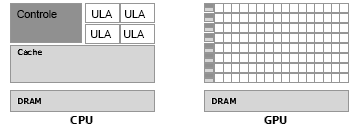
\includegraphics[width=1\textwidth]{imagens/gpu_1.png}
  \captionsource{As GPUs dedicam mais transistores ao processamento de dados}{\cite{CUDA}}
  \label{fig:gpu_1}
\end{figure}

Inicialmente o foco principal dessas placas era na industria de jogos e esse mercado bilionário impulsionou uma rápida evolução na capacidade das GPUs. Não demorou muito tempo para que os desenvolvedores em geral vissem que essas aplicações não são limitadas a industria de jogos. Inicialmente era muito trabalhoso aplicar a capacidade das placas de vídeo para aplicações gerais pois era necessário conhecer APIs especificas de processamento de imagem e saber traduzir os problemas de um domínio para o outro. Para que os desenvolvedores pudessem se aproveitar desse processamento para outros fins, os produtores de GPUs tem disponibilizado bibliotecas para executar operações de uso geral na GPU. Como o CUDA distribuído pela NVIDIA para ser usado em suas placas gráficas.

\section{CUDA}
Lançado em 2006 CUDA é plataforma de computação e modelo de programação proprietária da NVIDIA feita para desenvolvedores poderem explorar o potencial das suas GPUs para aplicações gerais, atualmente está na versão 7.5. CUDA foi desenvolvido para ser simples e facilmente compreensível por pessoas com familiaridade com linguagens de programação como C. Com o CUDA é possível enviar código em C, C++ e Fortran diretamente para GPU sem precisar escrever em assembly. 

%silvana: dizer de outra forma, que neste trabalho usaremos a API de CUDA para a linguagem C.
Nesse trabalho, não estarei abordando o uso do fortran.

A base do CUDA consiste de 3 abstrações: hierarquia de threads, memória compartilhada e sincronização. Essas abstrações estão acessíveis ao programador através de comandos básicos. 

%silvana: recolocar o trecho abaixo depois que você explicar o conceito de "bloco"
%A escalabilidade do CUDA é feita de forma transparente para o desenvolvedor, basta fazer o programa de forma realmente paralela onde um bloco não precise de informação de outro bloco e a ordem de execução não importa. A execução dos blocos é distribuída em tempo de execução de forma a explorar melhor a arquitetura.

\subsection{Modelo de programação}
O núcleo do CUDA consiste de kernels, 
%funções escritas em C 
que são funções especiais compiladas para serem executadas na GPU. O kernel é definido pela declaração $\_\_global\_\_$. O número de threads (fluxos de execução independente) %e blocos 
que vai executar a função é especificado quando a função é chamada pela sintaxe $nomeDaFuncao<<<blocos, threads>>>(parametros...)$. Blocos são conjuntos de threads que são executados no mesmo núcleo de processamento e compartilham uma área de memória específica de cada núcleo. 
%silvana: 

Atualmente nenhuma placa de vídeo suporta mais de 1024 threads por bloco, e esse valor precisa ser levado em consideração pelo desenvolvedor. Para executar a soma de dois vetores de 2048 elementos seria possível separar em 2 blocos de 1024 threads, 4 blocos de 512 threads ou 8 de 256, por exemplo. É recomendável que o número de threads por bloco seja múltiplo de 32, mas a proporção que vai dar o melhor resultado varia de aplicação para aplicação.
Para identificar qual thread vai processar qual dado, cada thread possui um id de thread, $threadIdx$, e de bloco, $blockIdx$, e é possível saber o índice do vetor que se quer acessar fazendo $indice = threadIdx.x + blockIdx.x * blockDim.x$, o $.x$ serve para identificar a dimensão que estamos acessando, é possivel enviar vetores de até 3 dimensões.
Cada kernel tem acesso a memória privada, compartilhada por bloco,  e global (compartilhada por todas as threads).

Em \ref{alg:cuda_1} apresentamos um exemplo de um kernel que eleva ao quadrado todos os elementos de um vetor. Mostramos como declarar um kernel, descobrir seu id para endereçar a posição correta do vetor e uma função que chama esse kernel no código.

\codec{Como escrever e chamar um Kernel}{alg:cuda_1}{codigos/cuda_1.txt}

%silvana: melhor dizer (depois de heterogênea...) que parte do programa executa na CPU (host) e outra parte na GPU (device)
%silvana: ok!
CUDA é um modelo de programação heterogênea onde parte do programa roda na CPU e outra parte na GPU. Para isso cada um executa um código distinto e possui memória distinta. Por isso é necessário no programa sequencial especificar para GPU como administrar a memória e quando executar os kernels. O CUDA oferece funções que permite a CPU dizer para GPU quando alocar memória, copiar dados para memória da GPU e executar os kernels.
A memoria pode ser alocada na GPU através de $cudaMalloc(\&dvcPtr, tamanho)$. É preciso salvar a referencia do ponteiro da GPU pois é esse ponteiro que vai ser passado para as chamadas de kernel. Para copiar informação do $host$ para o $device$ é preciso usar a função $cudaMemcpy(dvcPtr, hstPtr, tamanho,  tipo)$, tipo é um enum e pode ser $cudaMemcpyHostToDevice$ ou $cudaMemcpyHostToDevice$ entre outros. Para liberar a memória alocada no $device$ usa-se $cudaFree(devicePtr)$. 
As chamadas de CUDA para o $device$ pertencem à um stream, que funciona como uma fila que executa os comandos na ordem que foram chamadas. Algumas chamadas como as de kernel por default são assíncronas em relação ao $host$. Outras chamadas fazem a CPU eseperar a GPU terminar de trabalhar antes de continuar com o código. Como $cudaMemcpy(...)$ e $cudaDeviceSynchronize()$.

O programa descrito no código \ref{alg:cuda_2} utiliza muito dos conceitos que vimos. Como a alocação de memória no $device$, a cópia de um vetor do $host$ para o $device$, a chamada do kernel visto em \ref{alg:cuda_1}, a cópia de um vetor do $device$ para o $host$ e a liberação da memória alocada na GPU.

\codec{Como alocar memória e copiar dados para GPU}{alg:cuda_2}{codigos/cuda_2.txt}

Como as funções de CUDA não rodam na CPU as vezes é difícil saber o que está acontecendo e se ocorreu um erro ou se o programa está em um estado inválido do lado da GPU. Por isso as funções de cuda retornam códigos de erro ou sucesso definidos pelo enum $cudaError$. O kernel não possui esse retorno então é possível checar o status da GPU após as chamadas de kernel para saber se ocorreu um erro com a função $cudaGetLastError()$.

É possível incluir funções dentro de kernels de CUDA, para isso é preciso colocar a diretiva $\_\_device\_\_$ antes da função, assim o compilador vai saber que essa função deve ser executada em GPU e irá compilar de acordo. Caso queira que a função também possa rodar na CPU é possível colocar a diretiva $\_\_host\_\_$, assim usando as duas diretivas é possível usar a mesma função em códigos dentro e fora de kernels de CUDA.
